%%%%%%%%%%%%%%%%%%%%%%%%%%%%%%%%%%%%%%%%%
% Beamer Presentation
% LaTeX Template
% Version 1.0 (10/11/12) 
%
% This template has been downloaded from:
% http://www.LaTeXTemplates.com
%
% License:
% CC BY-NC-SA 3.0 (http://creativecommons.org/licenses/by-nc-sa/3.0/)
%
%%%%%%%%%%%%%%%%%%%%%%%%%%%%%%%%%%%%%%%%%

%----------------------------------------------------------------------------------------
%	PACKAGES AND THEMES
%----------------------------------------------------------------------------------------

\documentclass{beamer}

\mode<presentation> {
%\mode<handouts> {
%\mode<article> {


% The Beamer class comes with a number of default slide themes
% which change the colors and layouts of slides. Below this is a list
% of all the themes, uncomment each in turn to see what they look like.


%\usetheme{default}
%\usetheme{AnnArbor}
%\usetheme{Antibes}
%\usetheme{Bergen}
%\usetheme{Berkeley}
%\usetheme{Berlin}
%\usetheme{Boadilla}
\usetheme{CambridgeUS}
%\usetheme{Copenhagen}
%\usetheme{Darmstadt}
%\usetheme{Dresden}
%\usetheme{Frankfurt}
%\usetheme{Goettingen}
%\usetheme{Hannover}
%\usetheme{Ilmenau}
%\usetheme{JuanLesPins}
%\usetheme{Luebeck}
%\usetheme{Madrid}
%\usetheme{Malmoe}
%\usetheme{Marburg}
%\usetheme{Montpellier}
%\usetheme{PaloAlto}
%\usetheme{Pittsburgh}
%\usetheme{Rochester}
%\usetheme{Singapore}
%\usetheme{Szeged}
%\usetheme{Warsaw}

% As well as themes, the Beamer class has a number of color themes
% for any slide theme. Uncomment each of these in turn to see how it
% changes the colors of your current slide theme.

%\usecolortheme{albatross}
\usecolortheme{beaver}
%\usecolortheme{beetle}
%\usecolortheme{crane}
%\usecolortheme{dolphin}
%\usecolortheme{dove}
%\usecolortheme{fly}
%\usecolortheme{lily}
%\usecolortheme{orchid}
%\usecolortheme{rose}
%\usecolortheme{seagull}
%\usecolortheme{seahorse}
%\usecolortheme{whale}
%\usecolortheme{wolverine}

%\setbeamertemplate{footline} % To remove the footer line in all slides uncomment this line
%\setbeamertemplate{footline}[page number] % To replace the footer line in all slides with a simple slide count uncomment this line

%\setbeamertemplate{navigation symbols}{} % To remove the navigation symbols from the bottom of all slides uncomment this line
}

\usepackage{graphicx} % Allows including images
\graphicspath{{../figures}}
\usepackage{booktabs} % Allows the use of \toprule, \midrule and \bottomrule in tables
\usepackage{amsmath, amssymb, amsthm, gensymb,mathrsfs}%,eufrak}
\usepackage{hyperref}
\usepackage{tabularx}
\usepackage{longtable}
\usepackage{makecell}
\usepackage{multicol}
\usepackage{physics}

\newcommand{\uvec}[1]{\textbf{#1}}

\newcounter{excounter}
%\renewcommand{\thefpcounter}{\thechapter.\arabic{fpcounter}}
%\renewcommand{\thefpcounter}{\thesection.\arabic{fpcounter}}
\renewcommand{\theexcounter}{\arabic{excounter}}

\newtheorem{teorema}{Teorema}[section]
\newtheorem{definicio}{Definició}[section]

\usepackage[lastexercise]{exercise}

\graphicspath{{../figures}}

%----------------------------------------------------------------------------------------
%	 TITLE PAGE
%----------------------------------------------------------------------------------------

\title[Neural Networks]{Neural Networks} % The short title appears at the bottom of every slide, the full title is only on the title page

\author{Jordi Villà i Freixa} % Your name
\institute[FCTE] % Your institution as it will appear on the bottom of every slide, may be shorthand to save space
{
Universitat de Vic - Universitat Central de Catalunya \\
Study Abroad\\ % Your institution for the title page
\medskip
\textit{jordi.villa@uvic.cat} % Your email address
}
%\date{\today} % Date, can be changed to a custom date
\date{course 2023-2024}
\logo{
\includegraphics[width=.1\textwidth]{FCTE}}
\begin{document}

\begin{frame}
\titlepage % Print the title page as the first slide
\end{frame}

\begin{frame}
\frametitle{Index} % Table of contents slide, comment this block out to remove it
\tableofcontents % Throughout your presentation, if you choose to use \section{} and \subsection{} commands, these will automatically be printed on this slide as an overview of your presentation
\end{frame}

%----------------------------------------------------------------------------------------
%	PRESENTATION SLIDES
%----------------------------------------------------------------------------------------

%\subsection{Subsection Example} % A subsection can be created just before a set of slides with a common theme to further break down your presentation into chunks

\begin{frame}{What to expect?}
  In this session we will discuss:
  \begin{itemize}
    \item Neural networks
    \item Gradient Descent
    \item Backpropagation
  \end{itemize}
\end{frame}

\section{Neural Networks}


\begin{frame}{Tree-based methods}
\begin{itemize}
    \item Simple, intuitive and powerfiul for both regression and classification
    \item The method divides a feature space $X$ into smaller regions and fit a simple prediction function for each region.
    \begin{description}
        \item[Regression] eg, take the mean of the training responses associated with the training features that fall in the specific region
        \item[Classification] eg, take the majority vote among corresponding response variables.
    \end{description}
\end{itemize}
\end{frame}

\begin{frame}{Supervised ML}
    \begin{figure}
        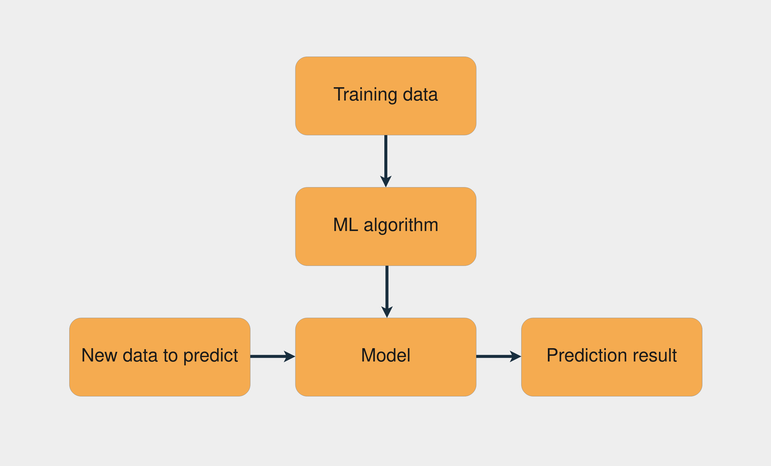
\includegraphics[width=0.9\linewidth]{ML}
        \caption{\href{https://realpython.com/python-ai-neural-network/}{Workflow} to train a model using supervised learning.}
        \label{Fig:ML}
    \end{figure}
\end{frame}

\begin{frame}{Feature engineering}
    \begin{figure}
        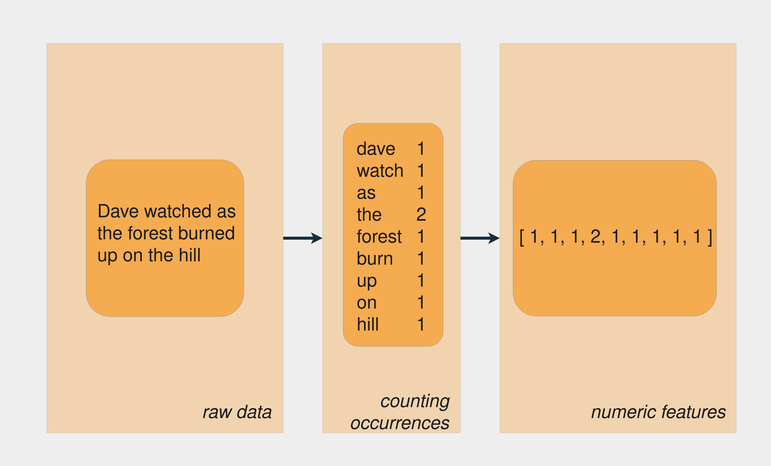
\includegraphics[width=0.9\linewidth]{FeatureEngineering}
        \caption{Feature engineering \href{https://realpython.com/python-ai-neural-network/}{example}.}
        \label{Fig:FeatureEngineering}
    \end{figure}
\end{frame}

\begin{frame}{Throwing darts and improving by learning}
    \begin{figure}
        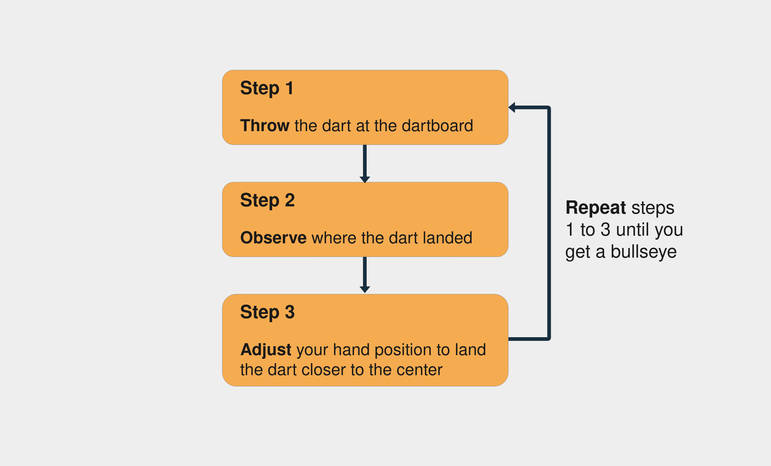
\includegraphics[width=0.9\linewidth]{TrainingDart}
        \caption{\href{https://realpython.com/python-ai-neural-network/}{Steps} for trying to hit the center of a dartboard.}
        \label{Fig:TrainingDart}
    \end{figure}
\end{frame}


\begin{frame}{An example of a 2 layer Neural Network}
    \begin{columns}
        \begin{column}{0.6\linewidth}     
            Example of classification (for categories "1" and "0") with a 2 layers NN. 
            \begin{itemize}
                \item In the first layer we use a linear regression approach.
                \item The second layer includes the non-linearity through the use of a sigmoid function that decides whether the prediction is 1 or 0.
            \end{itemize}
        \end{column}
        \begin{column}{0.4\linewidth}
            \begin{figure}
                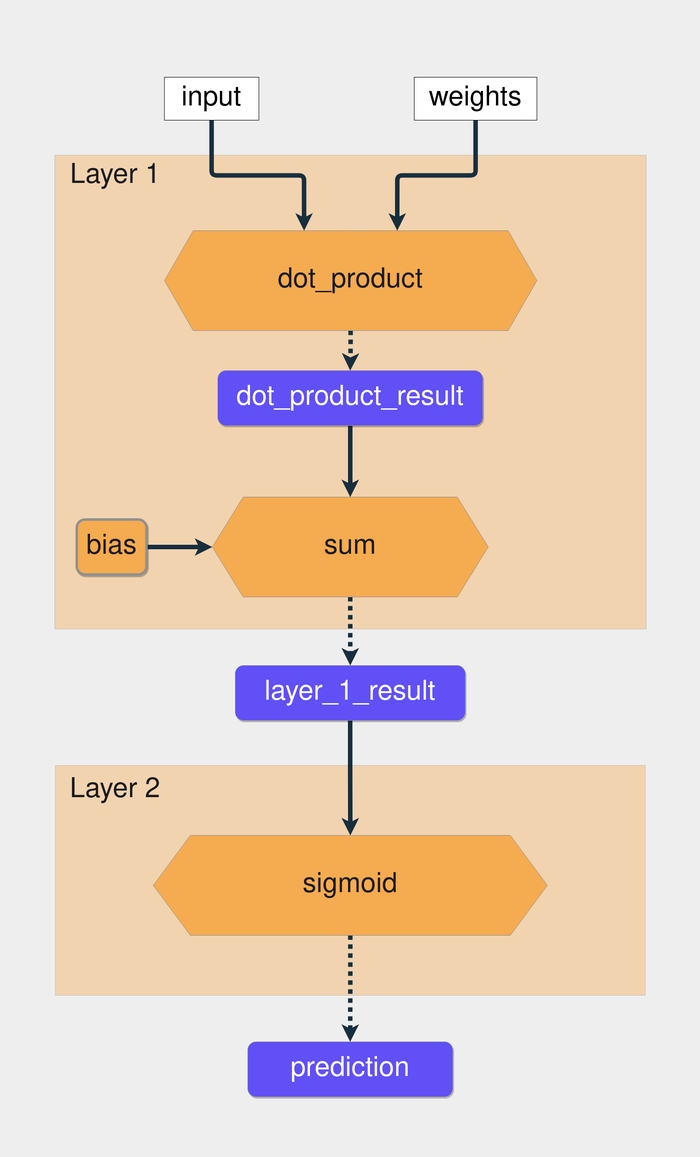
\includegraphics[width=0.7\linewidth]{Training2Layer}
                \caption{\href{https://realpython.com/python-ai-neural-network/}{Training} a two layer neural network.}
                \label{Fig:Training2Layer}
            \end{figure}
        \end{column}
     \end{columns}
\end{frame}

\begin{frame}
    \begin{Exercise}{Loss/Cost function in a simple 2 layer NN}
        \label{Ex:2layer}
        Check the provided code for this session
    \end{Exercise}
\end{frame}

\begin{frame}{Backpropagation: weights}
    \begin{columns}
        \begin{column}{0.6\linewidth}     
            {\bf Chain Rule in Backpropagation}In each {\bf backward pass}, you compute the partial derivatives of each function, substitute the variables by their values, and finally multiply everything.
            \\[10pt]
            Notice that, for the sigmoid function $f(x)=\frac{1}{1+e^{-x}}$, $f'(x)=1-f(x)$.
        \end{column}
        \begin{column}{0.4\linewidth}
            \begin{figure}
                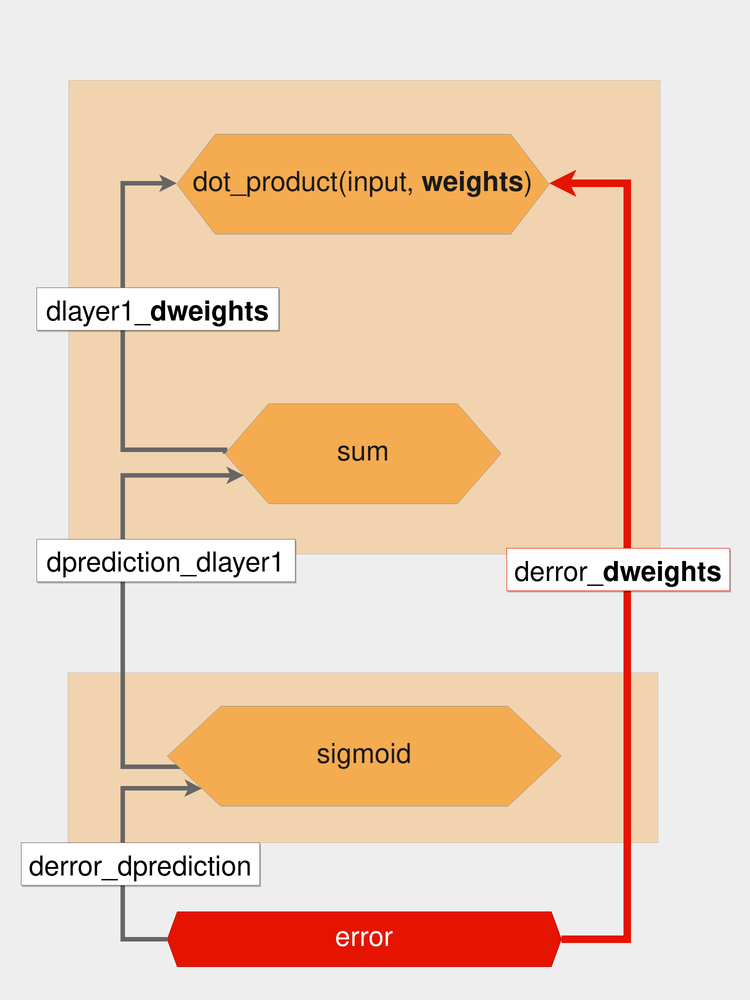
\includegraphics[width=0.7\linewidth]{WeightGradient.png}
                \caption{Chain rule to find the derivative of the {\bf error} with respect to the weights in the \href{https://realpython.com/python-ai-neural-network/}{2 layer NN}.}
                \label{Fig:Training2Layer}
            \end{figure}
        \end{column}
     \end{columns}
\end{frame}


\begin{frame}[fragile]{Backpropagation: Bias}
    \begin{columns}
        \begin{column}{0.6\linewidth}  
            Chain rule applied to the derivative of the bias error in the 2 layer example.   
            \begin{lstlisting}[language=Python]
derror_dbias = derror_dprediction * dprediction_dlayer1 * dlayer1_dbias
            \end{lstlisting}
        \end{column}
        \begin{column}{0.4\linewidth}
            \begin{figure}
                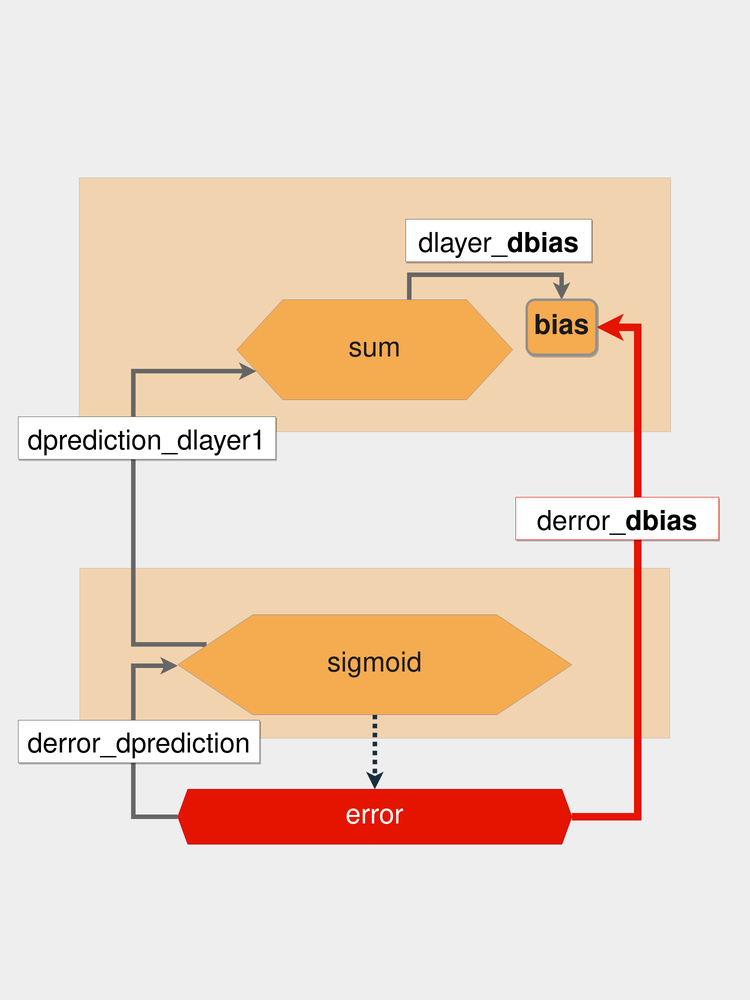
\includegraphics[width=0.7\linewidth]{BiasGradient}
                \caption{Chain rule to find the derivative of the {\bf bias} with respect to the weights in the \href{https://realpython.com/python-ai-neural-network/}{2 layer NN}.}
                \label{Fig:Training2Layer}
            \end{figure}
        \end{column}
     \end{columns}
\end{frame}

\begin{frame}
    \begin{figure}
        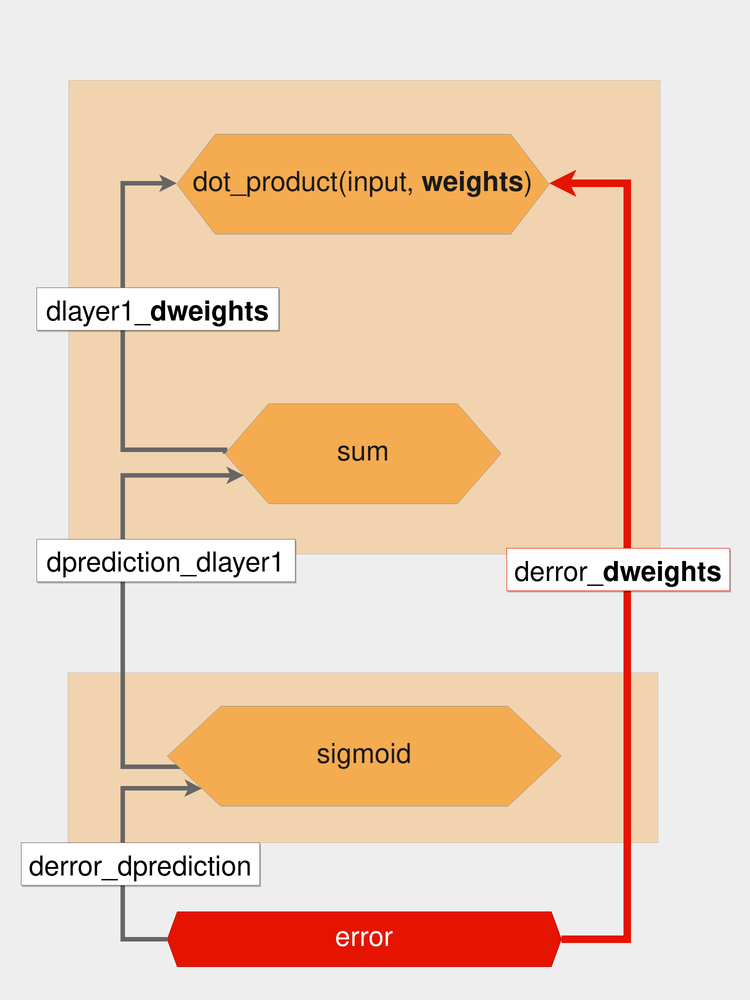
\includegraphics[width=0.9\linewidth]{WeightGradient}
        \caption{Left: training data and a new feature. Right: a partition of the feature space\cite{kroese2020}}
        \label{Fig:WeightGradient}
    \end{figure}
\end{frame}

\begin{frame}
    \begin{figure}
        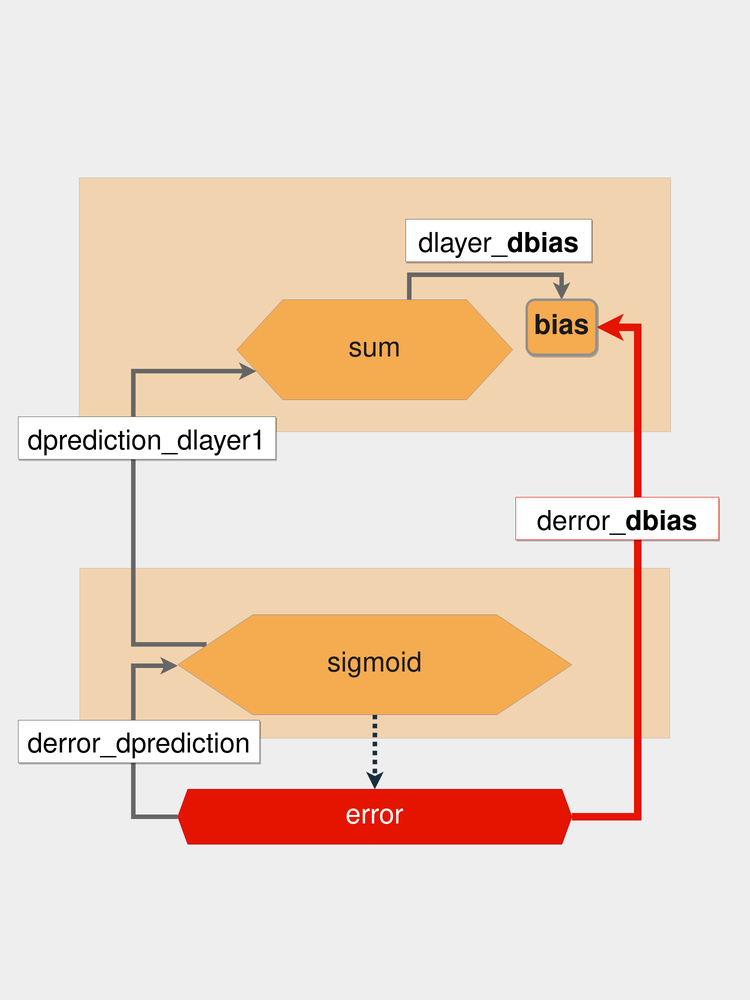
\includegraphics[width=0.9\linewidth]{BiasGradient}
        \caption{Left: training data and a new feature. Right: a partition of the feature space\cite{kroese2020}}
        \label{Fig:BiasGradient}
    \end{figure}
\end{frame}



\section{Bibliography}
\bibliographystyle{unsrt}
\bibliography{DataSciencewithPython}
\end{document}
